\documentclass[11pt]{article}
%Gummi|063|=)
\title{\textbf{Algorithms I -- supervision 6}}
\author{James Wood}
\usepackage{listings}
\usepackage{bold-extra}
\usepackage{xcolor}
\usepackage{amsmath}
\usepackage{enumitem}
\usepackage{tikz}
\usetikzlibrary{arrows}

\lstset{
  basicstyle=\small,
  basewidth=0.5em,
  frame=single,
  breaklines=true,
  %postbreak=\raisebox{0ex}[0ex][0ex]{
  %  \ensuremath{\color{red}\hookrightarrow\space}
  %}
  language=c++,
  literate=
    {<=}{{\(\leq\)}}1
    {>=}{{\(\geq\)}}1
    {&&}{{\(\wedge\)}}1
    {||}{{\(\vee\)}}1
    {->}{{\(\rightarrow\)}}1
}

\tikzset{
  treenode/.style = {align=center, inner sep=0pt, text centered,
    font=\sffamily},
  bnode/.style = {treenode, circle, white, draw=black,
    fill=black, text width=1.5em},
  rnode/.style = {treenode, circle, red, draw=red,
    text width=1.5em, very thick},
  leaf/.style = {treenode, rectangle, draw=black,
    minimum width=0.5em, minimum height=0.5em}
}

\begin{document}
\renewcommand{\labelenumi}{(\alph{enumi})}
\renewcommand{\labelenumii}{(\roman{enumii})}

\maketitle

\section{Dijkstra}
\begin{enumerate}
\item The algorithm starts at a given vertex, whose distance is marked as 0. All nodes directly connected to this vertex are added to a priority queue, sorted by weight of the connecting edge in ascending order (lightest first). The first vertex in the queue is then moved to, and is given a distance equal to the weight associated with it. Vertices directly conected to it without an assigned distance are then added to the queue, with value equal to the distance of the previous vertex plus the weight of the edge used to reach the new vertex, and the process is repeated. Assuming a connected graph, the algorithm terminates when all vertices have been assigned a distance, or equivalently when the queue is exhausted.
\item
  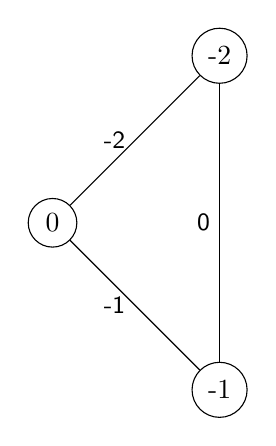
\begin{tikzpicture}[baseline={(1.base)},node distance=3cm,main node/.style={circle,draw}]
    \node[main node] (1) {-2};
    \node[main node] (2) [below left of=1] {0};
    \node[main node] (3) [below right of=2] {-1};

    \path[every node/.style={font=\sffamily\small}]
    (1) edge node [left] {-2} (2)
    (2) edge node [left] {-1} (3)
    (3) edge node [left] {0} (1);
  \end{tikzpicture}
\item Consider this graph:

  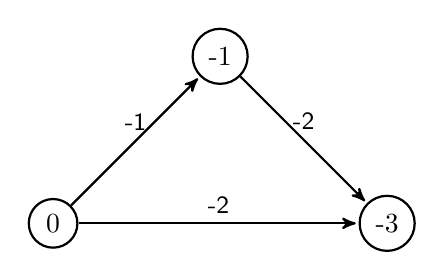
\begin{tikzpicture}[->,>=stealth',shorten >=1pt,auto,node distance=3cm,thick,main node/.style={circle,draw}]
    \node[main node] (0) {0};
    \node[main node] (1) [above right of=0] {-1};
    \node[main node] (2) [below right of=1] {-3};

    \path[every node/.style={font=\sffamily\small}]
    (0) edge node [above] {-1} (1)
    (1) edge node [above] {-2} (2)
    (0) edge node [above] {-2} (2);
  \end{tikzpicture}

  The shortest path from left to right goes via the middle node. Adding 2 to the weight of each arc gives this:

  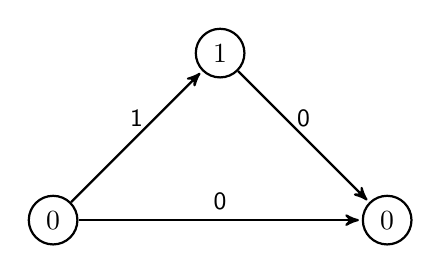
\begin{tikzpicture}[->,>=stealth',shorten >=1pt,auto,node distance=3cm,thick,main node/.style={circle,draw}]
    \node[main node] (0) {0};
    \node[main node] (1) [above right of=0] {1};
    \node[main node] (2) [below right of=1] {0};

    \path[every node/.style={font=\sffamily\small}]
    (0) edge node [above] {1} (1)
    (1) edge node [above] {0} (2)
    (0) edge node [above] {0} (2);
  \end{tikzpicture}

  The shortest path from left to right is now to go there directly. Hence, this tactic does not work.
\item
  \begin{enumerate}
    \item Inserting a vertex into the queue takes \(O\,1\) time, and is done \(O\,|E|\) times. Extracting a vertex takes \(O\,|V|\) time, and this is done \(O\,|V|\) times. These give the total complexity \(O\,(|E|+|V|^2)\), which is equivalent to just \(O\,(|V|^2)\).
    \item The estimate could be poor. Inserting now takes \(O\,|V|\) time, giving a total complexity of \(O\,(|V|\cdot|E|+|V|^2)\), which is simplified to \(O\,(|V|\cdot|E|)\).
    \item Inserting takes \(O\,(\log{|V|})\) time and extracting takes \(O\,(\log{|V|})\) time, giving complexity \(O\,(|E|\cdot\log{|V|}+|V|\cdot\log{|V|})\), which is \(O\,(|E|\cdot\log{|V|})\).
    \item Inserting/modifying costs \(O\,(\log{|V|})\), and extracting costs \(O\,(\log{|V|})\), giving the same complexity as the binary heap.
    \item Inserting/modifying has \(O\,1\) amortized cost, and extracting costs \(O\,(\log{|V|})\), giving complexity \(O\,(|E|+|V|\cdot\log{|V|})\).
  \end{enumerate}
\end{enumerate}

\section{Amortized and aggregate analysis}
\begin{enumerate}
\item Amortized analysis involves finding a worst-case sequence of instructions, analyzing the complexity of the sequence and dividing the cost of the sequence by the length of the sequence, yielding an average cost for each instruction. Aggregate analysis is done by creating a measure function for the given data structure, and giving the cost of each operation as its time complexity plus the change it causes in the measure of the data structure.
\item
  \begin{enumerate}
  \item The \texttt{multipush} operation can be run on any stack, and will always have cost \(n\), where \(n\) is the length of the list of items being pushed. Hence, its amortized cost is \(O\,n\).
  \item
    \begin{minipage}[t]{\linewidth}
      \begin{lstlisting}
class Queue
    Stack front
    Stack back

    void enqueue(Item x)
        back.push(x)

    Item dequeue()
        if front.isEmpty() then
            until back.isEmpty()
                front.push(back.pop())
        return front.pop()

    Boolean isEmpty()
        return front.isEmpty() && back.isEmpty()
      \end{lstlisting}
    \end{minipage}
  \item Let \(\phi\) be a function measuring the length of \texttt{back}. \texttt{enqueue} has time cost 1 plus potential cost 1. \texttt{dequeue} has either time cost 1 plus potential cost 0, or time cost \(n+1\) plus potential cost \(-n\). \texttt{isEmpty} has time cost 1 plus potential cost 0. Each of these possibilites give linear aggregate cost, so the amortized running time of each operation is linear.
  \end{enumerate}
\end{enumerate}

\section{Linear cost}
In the operation of the queue, it is always the case that either all of the items are in the correct place, or exactly one item is too high in priority for its position. The latter situation occurs after either an insertion to the start of the array or a call to \texttt{decreaseKey}. Keeping high-priority (low-key) items at the right, the out-of-place item is too far left. Bubble sort will move it to the correct position in one pass. If a standard bubble sort algorithm is used, there will also be another pass to check the array, but this doesn't affect asymptotic complexity.

\section{Disjoint-sets, linked lists and trees}
\begin{enumerate}
\item The disjoint-set data structure represents a collection of sets, with no two of those sets sharing any elements. Items can be queried as to which set they are in, and sets can be merged together (preserving all elements, since they are disjoint to each other).
\item Each subset is stored as a linked list, and these are all stored inside a linked list. This takes \(O\,n\) time to create, \(O\,n\) time to find elements and \(O\,(s+l)\) time to merge two subsets (where \(s\) is the number of subsets and \(l\) is the size of the first subset of the two being merged).
\item In Kruskal's algorithm, data representing each edge of the graph are put into a priority queue with lighter edges first. Also, data representing vertices are put into a disjoint-set data structure. Edges are taken from the priority queue and added to the output tree iff they connect vertices from different subsets. When an edge is added, the sets containing its vertices are merged. The algorithm terminates when there is only one disjoint set left.
\item At most \(|E|\) edges are chosen. If the edges are given in a sorted list (which took \(O\,(|E|\cdot\log{|E|})\) time to create), the edge is taken from the priority queue in constant time. The resulting computation consists of two \texttt{find}s and a \texttt{merge}, which combined can take \(O\,|V|\) time. In a connected graph, \(|V|\leq 2\cdot|E|\), so this is equivalent to \(O\,|E|\). Therefore, the total running time is \(O\,(|E|\cdot\log{|E|})\).
\end{enumerate}

\section{Recurrence relations}
\begin{enumerate}
\item Observe:
  \[
    \begin{aligned}
      T\,u&\leq 2\cdot T\,(u^{\frac{1}{2}})+c \quad &&\textrm{for some constant }c \\
      &\leq 2^k\cdot T\,\left(u^{\frac{1}{2^k}}\right)+\left(2^k-1\right)\cdot c \quad &&\textrm{for any }k\textrm{ small enough}
    \end{aligned}
  \]
  This can be verified by induction. Take the implicit base case to be \(T\,2=1\), and choose \(k\) such that:
  \[
    \begin{aligned}
      u^{\frac{1}{2^k}}&=2 \\
      u&=2^{2^k} \\
      \lg u&=2^k
    \end{aligned}
  \]
  Substituting this in, we get:
  \[
    \begin{aligned}
      T\,u&\leq\lg u\cdot T\,2+\left(\lg u-1\right)\cdot c \\
      &\leq(c+1)\cdot\lg u - c \\
      &\in O\,(\lg u) \quad \textrm{QED}
    \end{aligned}
  \]
\item Similarly, we find that:
  \[
    \begin{aligned}
      T\,u&\leq 2^k\cdot T\,\left(u^{\frac{1}{2^k}}\right)+c\cdot\lg\left(u^{\frac{k}{2}}\right) \quad &&\textrm{for some }c \\
      &\leq 2^k\cdot T\,\left(u^{\frac{1}{2^k}}\right)+\frac{c}{2}\cdot k\cdot\lg u
    \end{aligned}
  \]
  Again, try:
  \[
    \begin{aligned}
      u^{\frac{1}{2^k}}&=2 \\
      u&=2^{2^k} \\
      \lg u&=2^k \\
      \lg\,(\lg u)&=k
    \end{aligned}
  \]
  Using the last two results and the base case \(T\,2=1\), we rewrite the inequality as:
  \[
    \begin{aligned}
      T\,u&=\lg u+\frac{c}{2}\cdot\lg\,(\lg u)\cdot\lg u \\
      &\in O\,(\lg u\cdot\lg\,(\lg u)) \quad \textrm{QED}
    \end{aligned}
  \]
\end{enumerate}

\section{k-Anonymity}
\begin{enumerate}
\item Yes. There are an odd number of elements, so there had to be some group of three, which has a cost of at least 3. Pairings have a cost of at least 1. This solution incurred only those costs, so is optimal.
\item Let the length of the list be \(d\cdot k+r\), where \(r\in[0..k)\). Produce all possible partitionings of the list where the size of each partition is in \([k..2k)\). In each partition, increase all of the elements to become equal to the largest element, keeping track of the cost. Sum the costs from all partitions in each partitioning, and choose the partitioning with the lowest cost. This can be re\"assembled to give a valid output.

  This seems to have factorial cost, since almost all possible partitionings have to be checked exhaustively.
\item Some improvement can be gained by memoization, though this doesn't reach linear running time.
\end{enumerate}

\end{document}